% generated by Plantuml 1.2025.2       
\definecolor{plantucolor0000}{RGB}{241,241,241}
\definecolor{plantucolor0001}{RGB}{24,24,24}
\definecolor{plantucolor0002}{RGB}{0,0,0}
\definecolor{plantucolor0003}{RGB}{34,34,34}
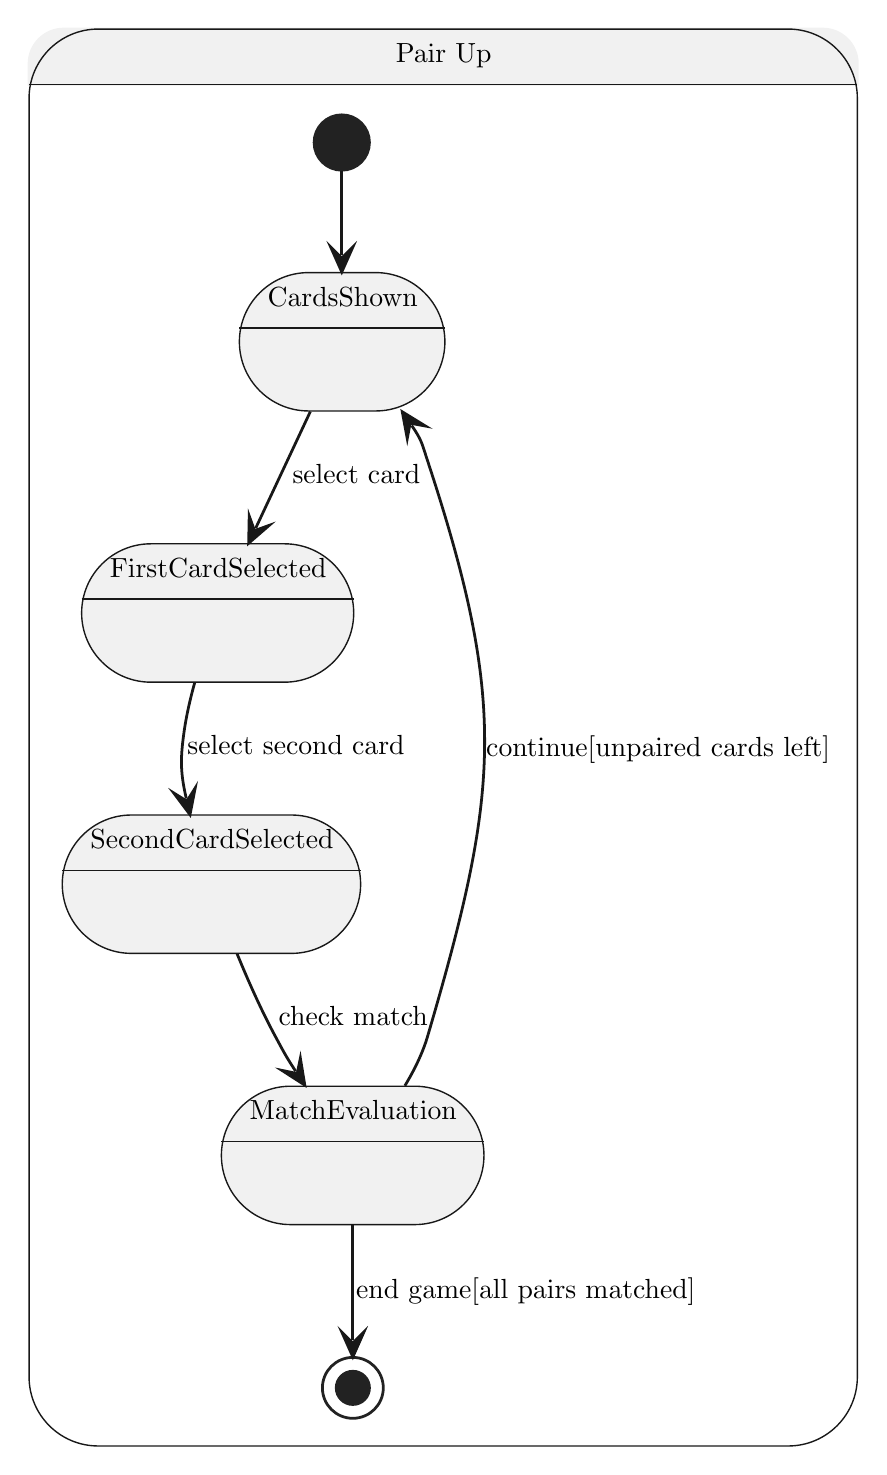
\begin{tikzpicture}[yscale=-1
,pstyle1/.style={color=plantucolor0001,line width=0.5pt}
,pstyle2/.style={color=plantucolor0003,fill=plantucolor0003,line width=1.0pt}
,pstyle3/.style={color=plantucolor0001,fill=plantucolor0000,line width=0.5pt}
,pstyle5/.style={color=plantucolor0001,line width=1.0pt}
,pstyle6/.style={color=plantucolor0001,fill=plantucolor0001,line width=1.0pt}
]
\draw[color=plantucolor0000,fill=plantucolor0000,line width=1.0pt] (19.5pt,7pt) -- (293.8pt,7pt) arc(270:360:12.5pt)  -- (306.3pt,27pt) -- (7pt,27pt) -- (7pt,19.5pt) arc(180:270:12.5pt) ;
\draw[pstyle1] (7pt,32pt) arc (180:270:25pt) -- (32pt,7pt) -- (281.3pt,7pt) arc (270:360:25pt) -- (306.3pt,32pt) -- (306.3pt,494pt) arc (0:90:25pt) -- (281.3pt,519pt) -- (32pt,519pt) arc (90:180:25pt) -- (7pt,494pt) -- cycle;
\draw[pstyle1] (7pt,27pt) -- (306.3pt,27pt);
\node at (139.34pt,12pt)[below right,color=black,inner sep=0]{Pair Up};
\draw[pstyle2] (120pt,48pt) ellipse (10pt and 10pt);
\draw[pstyle3] (83pt,120pt) arc (180:270:25pt) -- (108pt,95pt) -- (132.26pt,95pt) arc (270:360:25pt) -- (157.26pt,120pt) -- (157.26pt,120pt) arc (0:90:25pt) -- (132.26pt,145pt) -- (108pt,145pt) arc (90:180:25pt) -- (83pt,120pt) -- cycle;
\draw[pstyle1] (83pt,115pt) -- (157.26pt,115pt);
\node at (93pt,100pt)[below right,color=black,inner sep=0]{CardsShown};
\draw[pstyle3] (26pt,218pt) arc (180:270:25pt) -- (51pt,193pt) -- (99.31pt,193pt) arc (270:360:25pt) -- (124.31pt,218pt) -- (124.31pt,218pt) arc (0:90:25pt) -- (99.31pt,243pt) -- (51pt,243pt) arc (90:180:25pt) -- (26pt,218pt) -- cycle;
\draw[pstyle1] (26pt,213pt) -- (124.31pt,213pt);
\node at (36pt,198pt)[below right,color=black,inner sep=0]{FirstCardSelected};
\draw[pstyle3] (19pt,316pt) arc (180:270:25pt) -- (44pt,291pt) -- (101.81pt,291pt) arc (270:360:25pt) -- (126.81pt,316pt) -- (126.81pt,316pt) arc (0:90:25pt) -- (101.81pt,341pt) -- (44pt,341pt) arc (90:180:25pt) -- (19pt,316pt) -- cycle;
\draw[pstyle1] (19pt,311pt) -- (126.81pt,311pt);
\node at (29pt,296pt)[below right,color=black,inner sep=0]{SecondCardSelected};
\draw[pstyle3] (76.5pt,414pt) arc (180:270:25pt) -- (101.5pt,389pt) -- (146.38pt,389pt) arc (270:360:25pt) -- (171.38pt,414pt) -- (171.38pt,414pt) arc (0:90:25pt) -- (146.38pt,439pt) -- (101.5pt,439pt) arc (90:180:25pt) -- (76.5pt,414pt) -- cycle;
\draw[pstyle1] (76.5pt,409pt) -- (171.38pt,409pt);
\node at (86.5pt,394pt)[below right,color=black,inner sep=0]{MatchEvaluation};
\draw[color=plantucolor0003,line width=1.0pt] (124pt,498pt) ellipse (11pt and 11pt);
\draw[pstyle2] (124pt,498pt) ellipse (6pt and 6pt);
\draw[pstyle5] (120pt,58.15pt) ..controls (120pt,67.42pt) and (120pt,76.14pt) .. (120pt,88.78pt);
\draw[pstyle6] (120pt,94.78pt) -- (124pt,85.78pt) -- (120pt,89.78pt) -- (116pt,85.78pt) -- (120pt,94.78pt) -- cycle;
\draw[pstyle5] (108.64pt,145.22pt) ..controls (101.82pt,159.78pt) and (95.7165pt,172.7972pt) .. (88.8965pt,187.3472pt);
\draw[pstyle6] (86.35pt,192.78pt) -- (93.7916pt,186.3285pt) -- (88.4721pt,188.2527pt) -- (86.5479pt,182.9331pt) -- (86.35pt,192.78pt) -- cycle;
\node at (102pt,164pt)[below right,color=black,inner sep=0]{select card};
\draw[pstyle5] (66.85pt,243.18pt) ..controls (65.25pt,248.95pt) and (63.82pt,255.14pt) .. (63pt,261pt) ..controls (61.62pt,270.82pt) and (61.6759pt,275.7225pt) .. (63.8159pt,285.0325pt);
\draw[pstyle6] (65.16pt,290.88pt) -- (67.0422pt,281.2127pt) -- (64.0399pt,286.0071pt) -- (59.2455pt,283.0048pt) -- (65.16pt,290.88pt) -- cycle;
\node at (64pt,262pt)[below right,color=black,inner sep=0]{select second card};
\draw[pstyle5] (82.15pt,341.1pt) ..controls (86.04pt,350.61pt) and (90.87pt,361.5pt) .. (96pt,371pt) ..controls (99.17pt,376.86pt) and (99.6308pt,377.9219pt) .. (103.3408pt,383.5819pt);
\draw[pstyle6] (106.63pt,388.6pt) -- (105.0415pt,378.8801pt) -- (103.889pt,384.4183pt) -- (98.3508pt,383.2657pt) -- (106.63pt,388.6pt) -- cycle;
\node at (97pt,360pt)[below right,color=black,inner sep=0]{check match};
\draw[pstyle5] (142.8pt,388.83pt) ..controls (146.17pt,383.26pt) and (149.19pt,377.15pt) .. (151pt,371pt) ..controls (177.05pt,282.3pt) and (179.9pt,250.81pt) .. (151pt,163pt) ..controls (148.96pt,156.8pt) and (149.0188pt,155.7145pt) .. (145.2588pt,150.2445pt);
\draw[pstyle6] (141.86pt,145.3pt) -- (143.6618pt,154.9826pt) -- (144.6923pt,149.4204pt) -- (150.2545pt,150.4509pt) -- (141.86pt,145.3pt) -- cycle;
\node at (172pt,262pt)[below right,color=black,inner sep=0]{continue[unpaired cards left]};
\draw[pstyle5] (124pt,439.16pt) ..controls (124pt,455.03pt) and (124pt,468.98pt) .. (124pt,480.82pt);
\draw[pstyle6] (124pt,486.82pt) -- (128pt,477.82pt) -- (124pt,481.82pt) -- (120pt,477.82pt) -- (124pt,486.82pt) -- cycle;
\node at (125pt,458pt)[below right,color=black,inner sep=0]{end game[all pairs matched]};
\end{tikzpicture}
